\newif\ifimagen\imagentrue
\documentclass{article}
\usepackage[latin1]{inputenc}
\usepackage{alltt,hevea,color,amsmath,amssymb,prooftree}
\usepackage{fancyheadings}
\usepackage[latin1]{inputenc}
\usepackage{graphicx,multicol,amsmath,amssymb,ifthen}
\newcommand{\mtt}{\color{Gray}\tt}
\newcommand{\letml}{{\color{OliveGreen}let}}
\newcommand{\andml}{{\color{OliveGreen}and}}
\newcommand{\inml}{{\color{OliveGreen}in}}
\newcommand{\letrecml}{{\color{OliveGreen}let rec}}
\newcommand{\funml}{{\color{OliveGreen}function}}
\newcommand{\ifml}{{\color{OliveGreen}if}}
\newcommand{\thenml}{{\color{OliveGreen}then}}
\newcommand{\typeml}{{\color{OliveGreen}type}}
\newcommand{\ofml}{{\color{OliveGreen}of}}
\newcommand{\elseml}{{\color{OliveGreen}else}}
\newcommand{\matchml}{{\color{OliveGreen}match}}
\newcommand{\withml}{{\color{OliveGreen}with}}
\newcommand{\tr}[3]{%
\begin{toimage}
$\displaystyle\frac{#1}{#2}\ #3$
\end{toimage}\imageflush}
\newcommand{\prf}[1]{%
\begin{toimage}
  \begin{center}
    \begin{tabular}{c}
    \mbox{\input{#1}}
    \end{tabular}
  \end{center}
\end{toimage}\imageflush}
\newcommand{\imp}{\Rightarrow}
\newcommand{\blanc}{\quad\quad}
\newcommand{\im}[1]{%
\begin{toimage}
$#1$
\end{toimage}\imageflush}

\pagestyle{empty}
\thispagestyle{empty}
\begin{document}

$A\Rightarrow\bot$

\clearpage% page: 0

$\neg A$

\clearpage% page: 1

$A\vee\neg A$

\clearpage% page: 2

$\Gamma\vdash f$

\clearpage% page: 3

$f\in\Gamma$

\clearpage% page: 4
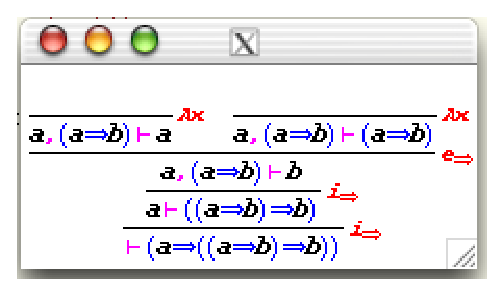
\includegraphics[width=5.5cm]{exemple1.ps}
\clearpage% page: 5

$\Gamma\vdash A\wedge B$

\clearpage% page: 6

$\Gamma\vdash A$

\clearpage% page: 7

$\Gamma\vdash B$

\clearpage% page: 8

$\vdash (a\Rightarrow ((a\Rightarrow b) \Rightarrow b))$

\clearpage% page: 9

$\vdash (a\Rightarrow b) \Rightarrow ((b\Rightarrow c)\Rightarrow (a\Rightarrow c))$

\clearpage% page: 10

$\vdash (a\Rightarrow(b\Rightarrow c)) \Rightarrow ((a\Rightarrow b)\Rightarrow (a\Rightarrow c))$

\clearpage% page: 11

$\vdash (a\vee b) \Rightarrow ((a\Rightarrow b)\Rightarrow b)$

\clearpage% page: 12

$\vdash (a\vee(b\wedge c))\Rightarrow((a\vee b)\wedge(a\vee c))$

\clearpage% page: 13

$\vdash \neg a \Rightarrow ((a\vee b)\Rightarrow b)$

\clearpage% page: 14

$\vdash (a \Rightarrow b) \Rightarrow (\neg b\Rightarrow \neg a)$

\clearpage% page: 15

$\vdash (\neg b\Rightarrow \neg a) \Rightarrow (a \Rightarrow b)$

\clearpage% page: 16

$\vdash  (\neg a\vee b) \Rightarrow (a \Rightarrow b)$

\clearpage% page: 17

$\vdash  (a \Rightarrow b) \Rightarrow (\neg a\vee b)$

\clearpage% page: 18

$\vdash  \neg (a\vee b) \Rightarrow (\neg a \wedge \neg b)$

\clearpage% page: 19

$\vdash  \neg (a\wedge b) \Rightarrow (\neg a \vee \neg b)$

\clearpage% page: 20

$\vdash (\neg a \vee \neg b) \Rightarrow \neg (a\wedge b)$

\clearpage% page: 21

$\vdash (\neg a \wedge \neg b) \Rightarrow \neg (a\vee b)$

\clearpage% page: 22

  \begin{center}
    \begin{tabular}{c}
    \mbox{\introimp{ \vdash (a \Rightarrow b) \Rightarrow ((a \Rightarrow b) \wedge b) \Rightarrow b}{\lemme{et1}{a \Rightarrow b \vdash ((a \Rightarrow b) \wedge b) \Rightarrow b}}


}
    \end{tabular}
  \end{center}

\clearpage% page: 23

  \begin{center}
    \begin{tabular}{c}
    \mbox{\introimp{ \vdash (p \wedge q) \Rightarrow q}{\elimet2{p \wedge q \vdash q}{\ax{p \wedge q \vdash p \wedge q}}}


}
    \end{tabular}
  \end{center}

\clearpage% page: 24

$[p\mapsto a\wedge b,q\mapsto b]$

\clearpage% page: 25

$[p\mapsto a\wedge b,p\mapsto b]$

\clearpage% page: 26

$a\wedge (b\vee a)$

\clearpage% page: 27

$c\wedge ((a\imp b)\vee c)$

\clearpage% page: 28

$a\wedge (b\vee a)$

\clearpage% page: 29

$c\wedge ((a\imp b)\vee a)$

\clearpage% page: 30
%Options: 
\end{document}
